\subsection{Häufige Funktionsgraphen}
    \subsubsection{ln(x)}
    \centerline{
        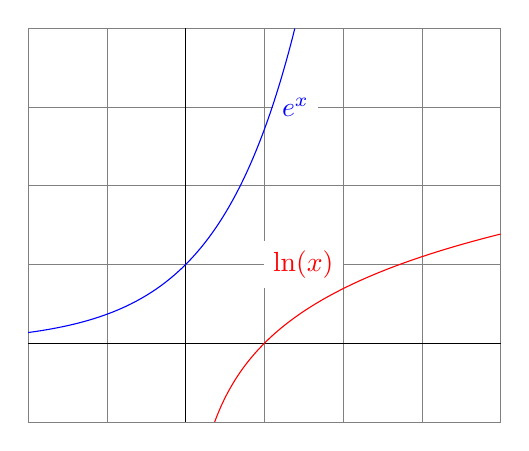
\begin{tikzpicture}
            \draw [help lines] (-2,-1) grid [step=1] (4,4);
            \draw (-2,0) -- (4,0);
            \draw (0,-1) -- (0,4);
            \draw [color = red] plot [smooth, samples = 100, domain = 0.368:4] (\x, {ln(\x)});
                \draw (1.1,3) node[right, blue,fill=white] {$e^x$};
            \draw [color = blue] plot [smooth, samples = 100, domain = -2:1.386] (\x, {e^\x});
                \draw (2,1) node[left, red,fill=white] {$\ln(x)$};
        \end{tikzpicture}
    }